\documentclass[a4paper,adobefonts,11pt,UTF8]{book}

%type chinese characters
\usepackage{ctex}

%Bibliography
\usepackage{chapterbib}
\usepackage[sectionbib,square,super,sort&compress]{natbib}


%generate index of book
\usepackage{makeidx}

%modify the headheight at least 13.5pt
\usepackage[headheight=13.6pt]{geometry}

%
\usepackage{fontspec}

%unicode
\usepackage{xunicode}

%
\usepackage{xltxtra}

%mathematics package
\usepackage{amsmath}

%mathematics symbols
\usepackage{amssymb}

%origin print package
\usepackage{verbatim}

%draw graphics use tikz and so on.
\usepackage{graphicx}

%set graphics path which used in the book.
\graphicspath{{../img/}}

%colorful table
\usepackage{colortbl}

%set color use origin name directly.
\usepackage[svgnames,table]{xcolor}

%
\usepackage[figuresright]{rotating}

% generate longtable which could across pages.
\usepackage{longtable}

\usepackage{lscape}

%
\usepackage{multirow}

%
\usepackage{adjustbox}


%
\newcommand\mgape[1]{\gape{$\vcenter{\hbox{#1}}$}}

%
\usepackage{array}

%
\usepackage{makecell}

%
\usepackage{ulem}

%
\usepackage{color}

% draw graphics use tikz package
\usepackage{tikz}

%
\usepackage{listings}
\lstset{
  basicstyle=\ttfamily,
  showstringspaces=false,
  commentstyle=\color{red},
  keywordstyle=\color{blue},
  columns=flexible,
  backgroundcolor=\color{lightgray},
  extendedchars=true,
  basicstyle=\footnotesize\ttfamily,
  showstringspaces=false,
  showspaces=false,
  numbers=left,
  numberstyle=\footnotesize,
  numbersep=9pt,
  tabsize=2,
  breaklines=true,
  showtabs=false,
  captionpos=b
}

%
\usepackage{bashful}

%set book information including bookmarksnumbered,pdfencoding,
%pdfauthor,pdfpagelayout,breaklinks,colorlinks,linkcolor,
%urlcolor,and so on.
\usepackage[bookmarksnumbered,pdfencoding=auto,pdfauthor={穷屌丝联盟},pdfpagelayout=TwoPageRight,breaklinks,colorlinks,linkcolor=RoyalBlue,urlcolor=blue,colorlinks=true]{hyperref}

%add more list types.
\usepackage{paralist}

%set page styles
\usepackage{fancyhdr}

\pagestyle{fancy}
\fancyhf{}
\fancyhead[LE,RO]{\thepage}
\fancyhead[RE]{\leftmark}
\fancyhead[RO]{\rightmark}
\fancypagestyle{plain}{
  \fancyhf{}
  \renewcommand{\headrulewidth}{0pt}
}


%titlepage \titleGM
\newcommand*{\plogo}{\fbox{$\mathcal{PL}$}} % Generic publisher logo
%--------------------------------------------------------------------
% TITLE PAGE
%--------------------------------------------------------------------

\newcommand*{\titleGM}{\begingroup % Create the command for including the title page in the document
\hbox{ % Horizontal box
\hspace*{0.2\textwidth} % Whitespace to the left of the title page
\rule{1pt}{\textheight} % Vertical line
\hspace*{0.05\textwidth} % Whitespace between the vertical line and title page text
\parbox[b]{0.75\textwidth}{ % Paragraph box which restricts text to less than the width of the page
{\noindent\Huge\bfseries Notes Collection of \\[0.5\baselineskip] Web Development}\\[2\baselineskip] % Title
{\large \textit{Web Development}}\\[4\baselineskip] % Tagline or further description
{\Large \textsc{theqiong.com}} % Author name

\vspace{0.5\textheight} % Whitespace between the title block and the publisher
{\noindent 穷屌丝联盟}\\[\baselineskip] % Publisher and logo
}}
\endgroup}
%


%lstlisting[language=JavsScript]
% Taken from Lena Herrmann at 
% http://lenaherrmann.net/2010/05/20/javascript-syntax-highlighting-in-the-latex-listings-package
\definecolor{lightgray}{rgb}{.9,.9,.9}
\definecolor{darkgray}{rgb}{.4,.4,.4}
\definecolor{purple}{rgb}{0.65,0.12,0.82}

%lstlisting package -----------
% JavaScript
%------------------------------
\lstdefinelanguage{JavaScript}
{
  keywords={typeof,new,ture,false,catch,function,return,null,switch,var,if,in,while,do,else,case,break},
  keywordstyle=\color{blue}\bfseries,
  ndkeywords={class,export,boolean,throw,implements,import,this},
  ndkeywordstyle=\color{darkgray}\bfseries,
  identifierstyle=\color{black},
  sensitive=false,
  comment=[l]{//},
  morecomments[s]{/*}{*/},
  commentstyle=\color{purple}\ttfamily,
  stringstyle=\color{red}\ttfamily,
  morestring=[b]',
  morestring=[b]"
}

\lstdefinelanguage{Scheme}
{morekeywords={,lambda, cond, case, display, let, import, quote, quasiquote, unquote,
define, begin, newline, if, list, apply, null?, car, cdr, or, not, and, for-each, 
make-vector, vector-length, vector-ref, vector-set!, eqv?, eq?, equal?, else, set!, 
define-record-type, fields, mutable, immutable, assert, parent, with-exception-handler, }
sensitive=false,
morecomment=[l]{;},
morecomment=[s]{/*}{*/},
morestring=[b]",
}

\lstdefinelanguage{CSS}{
  morekeywords={accelerator,azimuth,background,background-attachment,
    background-color,background-image,background-position,
    background-position-x,background-position-y,background-repeat,
    behavior,border,border-bottom,border-bottom-color,
    border-bottom-style,border-bottom-width,border-collapse,
    border-color,border-left,border-left-color,border-left-style,
    border-left-width,border-right,border-right-color,
    border-right-style,border-right-width,border-spacing,
    border-style,border-top,border-top-color,border-top-style,
    border-top-width,border-width,bottom,caption-side,clear,
    clip,color,content,counter-increment,counter-reset,cue,
    cue-after,cue-before,cursor,direction,display,elevation,
    empty-cells,filter,float,font,font-family,font-size,
    font-size-adjust,font-stretch,font-style,font-variant,
    font-weight,height,ime-mode,include-source,
    layer-background-color,layer-background-image,layout-flow,
    layout-grid,layout-grid-char,layout-grid-char-spacing,
    layout-grid-line,layout-grid-mode,layout-grid-type,left,
    letter-spacing,line-break,line-height,list-style,
    list-style-image,list-style-position,list-style-type,margin,
    margin-bottom,margin-left,margin-right,margin-top,
    marker-offset,marks,max-height,max-width,min-height,
    min-width,-moz-binding,-moz-border-radius,
    -moz-border-radius-topleft,-moz-border-radius-topright,
    -moz-border-radius-bottomright,-moz-border-radius-bottomleft,
    -moz-border-top-colors,-moz-border-right-colors,
    -moz-border-bottom-colors,-moz-border-left-colors,-moz-opacity,
    -moz-outline,-moz-outline-color,-moz-outline-style,
    -moz-outline-width,-moz-user-focus,-moz-user-input,
    -moz-user-modify,-moz-user-select,orphans,outline,
    outline-color,outline-style,outline-width,overflow,
    overflow-X,overflow-Y,padding,padding-bottom,padding-left,
    padding-right,padding-top,page,page-break-after,
    page-break-before,page-break-inside,pause,pause-after,
    pause-before,pitch,pitch-range,play-during,position,quotes,
    -replace,richness,right,ruby-align,ruby-overhang,
    ruby-position,-set-link-source,size,speak,speak-header,
    speak-numeral,speak-punctuation,speech-rate,stress,
    scrollbar-arrow-color,scrollbar-base-color,
    scrollbar-dark-shadow-color,scrollbar-face-color,
    scrollbar-highlight-color,scrollbar-shadow-color,
    scrollbar-3d-light-color,scrollbar-track-color,table-layout,
    text-align,text-align-last,text-decoration,text-indent,
    text-justify,text-overflow,text-shadow,text-transform,
    text-autospace,text-kashida-space,text-underline-position,top,
    unicode-bidi,-use-link-source,vertical-align,visibility,
    voice-family,volume,white-space,widows,width,word-break,
    word-spacing,word-wrap,writing-mode,z-index,zoom},
  morestring=[s]{:}{;},
  sensitive,
  morecomment=[s]{/*}{*/}
}








\setmainfont[Mapping=tex-text]{Minion Pro}

\makeindex\makeindex


\title{Web Development Notes}
\author{穷屌丝联盟\\ \texttt{theqiong.com}}
\date{\today}

\begin{document}

\begin{titlepage}
\addcontentsline{toc}{part}{Cover}

\pagestyle{empty} % Removes page numbers

\titleGM % This command includes the title page


\end{titlepage}

\maketitle
\tableofcontents
\listoffigures
\listoftables
\printindex


\part{Introduction}



Web development\cite{web_development} is a broad term for the work involved in developing a web site for the Internet (World Wide Web) or an intranet (a private network). Web development can range from developing the simplest static single page of plain text to the most complex web-based internet applications, electronic businesses, and social network services. A more comprehensive list of tasks to which web development commonly refers, may include web design, web content development, client liaison, client-side/server-side scripting, web server and network security configuration, and e-commerce development. Among web professionals, "web development" usually refers to the main non-design aspects of building web sites: writing markup and coding.

For larger organizations and businesses, web development teams can consist of hundreds of people (web developers). Smaller organizations may only require a single permanent or contracting webmaster, or secondary assignment to related job positions such as a graphic designer and/or information systems technician. Web development may be a collaborative effort between departments rather than the domain of a designated department..

Since the commercialization of the web, web development has been a growing industry. The growth of this industry is being pushed especially by businesses wishing to sell products and services to online customers.


For tools and platforms, the public can use many open source systems to aid in web development. A popular example, the LAMP (Linux, Apache, MySQL, PHP) stack is available for download online free of charge. This has kept the cost of learning web development to a minimum. Another contributing factor to the growth of the industry has been the rise of easy-to-use WYSIWYG web-development software, most prominently Adobe Dreamweaver, WebDev, and Microsoft Expression Studio. Using such software, virtually anyone can relatively quickly learn to develop a very basic web page. Knowledge of HyperText Markup Language (HTML) or of programming languages is still required to use such software, but the basics can be learned and implemented quickly with the help of help files, technical books, internet tutorials, or face-to-face training.

An ever growing set of tools and technologies have helped developers build more dynamic and interactive websites. Web developers now help to deliver applications as web services which were traditionally only available as applications on a desk-based computer.

Instead of running executable code on a local computer, users can interact with online applications to create new content. This has created new methods in communication[citation needed] and allowed for many opportunities to decentralize information and media distribution. Users can interact with applications from many locations, instead of being tied to a specific workstation for their application environment.

Examples of dramatic transformation in communication and commerce led by web development include e-commerce. Online auction-sites such as eBay have changed the way consumers find and purchase goods and services. Online retailers such as Amazon.com and Buy.com (among many others) have transformed the shopping and bargain-hunting experience for many consumers. Another good example of transformative communication led by web development is the blog. Web applications such as WordPress and Movable Type have created easily-implemented blog-environments for individual web sites. The popularity of open-source content management systems such as Joomla!, Drupal, XOOPS, and TYPO3 and enterprise content management systems such as Alfresco have extended web development's impact at online interaction and communication.

Web development has also impacted personal networking and marketing. Websites are no longer simply tools for work or for commerce, but serve more broadly for communication and social networking. Websites such as Facebook and Twitter provide users with a platform to communicate and organizations with a more personal and interactive way to engage the public.

Web开发是指使用网页设计程序语言设计交互式的网页,又称动态网页,动态网页是指网页的内容是否可根据某种条件的改变而自动改变,如计数器就是动态的,当有人点击我们的网页时,计数器的值会自动增加;BBS论坛也是动态的,当用户在论坛上发布信息时,网页内容会自动更新,显示出新发布的信息及相关回复;等等。需要注意的是GIF动画和Flash动画是静态的。因为,这些动画一旦制作完成后,就不会再改变了,尽管Flash动画可以响应用户的事件。


Web Development can be split into many areas and a typical and basic web development hierarchy might consist of:

\begin{compactitem}
\item Client side coding

\begin{compactitem}
\item \href{http://en.wikipedia.org/wiki/Ajax_(programming)}{Ajax}

Asynchronous JavaScript provides new methods of using JavaScript, and other languages to improve the user experience.
\item \href{http://en.wikipedia.org/wiki/Adobe_Flash}{Flash}

Adobe Flash Player is a ubiquitous browser plugin ready for RIAs. Flex 2 is also deployed to the Flash Player (version 9+).
\item \href{http://en.wikipedia.org/wiki/JavaScript}{JavaScript}

JavaScript is a ubiquitous client side platform for creating and delivering rich web applications that can also run across a wide variety of devices. It is a dialect of the scripting language ECMAScript.
\item \href{http://en.wikipedia.org/wiki/JQuery}{jQuery}

Cross-browser JavaScript library designed to simplify and speed up the client-side scripting of HTML.
\item \href{http://en.wikipedia.org/wiki/Microsoft_Silverlight}{Microsoft Silverlight}

Microsoft's browser plugin that enables animation, vector graphics and high-definition video playback, programmed using XAML and .NET programming languages.
\item \href{http://en.wikipedia.org/wiki/HTML5}{HTML5} and \href{http://en.wikipedia.org/wiki/CSS3}{CSS3}

Latest HTML proposed standard combined with the latest proposed standard for CSS natively supports much of the client-side functionality provided by other frameworks such as Flash and Silverlight
\end{compactitem}

Looking at these items from an "umbrella approach", client side coding such as XHTML is executed and stored on a local client (in a web browser) whereas server side code is not available to a client and is executed on a web server which generates the appropriate XHTML which is then sent to the client. The nature of client side coding allows you to alter the HTML on a local client and refresh the pages with updated content (locally), web designers must bear in mind the importance and relevance to security with their server side scripts. If a server side script accepts content from a locally modified client side script, the web development of that page is poorly sanitized with relation to security.

\item Server side coding

\begin{compactitem}
\item ASP (Microsoft proprietary)
\item ActiveVFP (open source)
\item CSP, Server-Side ANSI C
\item ColdFusion (Adobe proprietary, formerly Macromedia, formerly Allaire)
\item CGI
\item Erlang, with Linux, Yaws, Mnesia, Erlang (LYME) solution stack
\item Groovy, using the Grails framework
\item Java, e.g. Java EE or WebObjects
\item Lotus Domino
\item Node.js
\item Perl, e.g. Catalyst, Dancer or Mojolicious (all open source)
\item PHP (open source)
\item Python, e.g. Django (web framework) (open source)
\item Real Studio Web Edition
\item Ruby, e.g. Ruby on Rails (open source)
\item Smalltalk e.g. Seaside, AIDA/Web
\item SSJS Server-Side JavaScript, e.g. Aptana Jaxer, Mozilla Rhino
\item WebDNA (WSC proprietary)
\item Websphere (IBM proprietary)
\item .NET and .NET MVC Frameworks (Microsoft proprietary)
\end{compactitem}


\item Client side + server side

\begin{compactitem}
\item Google Web Toolkit provides tools to create and maintain complex JavaScript front-end applications in Java.
\item Dart provides tools to create and maintain complex JavaScript front-end applications as well as supporting server-side code in Dart (programming language).
\item Opa is a high-level language in which both the client and the server parts are implemented. The compiler then decides which parts run on the client (and are translated automatically to JavaScript) and which parts run on the server. The developer can tune those decisions with simple directives. (open source)
\item Pyjamas is a tool and framework for developing Ajax applications and Rich Internet Applications in python.
\item Tersus is a platform for the development of rich web applications by visually defining user interface, client side behavior and server side processing. (open source)
\end{compactitem}

However languages like Ruby and Python are often paired with database servers other than MySQL (the M in LAMP). Below are example of other databases currently in wide use on the web. For instance some developers prefer a LAPR(Linux/Apache/PostgreSQL/Ruby on Rails) setup for development.

\item Database technology

\begin{compactitem}
\item FileMaker
\item Apache Derby
\item IBM DB2
\item Firebird
\item Microsoft SQL Server
\item MySQL
\item Oracle
\item PostgreSQL
\item SQLite
\item Sybase
\item WebDNA
\item Redis
\item MongoDB
\item CouchDB
\item Mark\_Logic
\end{compactitem}


\end{compactitem}

The World Wide Web has become a major delivery platform for web development a variety of complex and sophisticated enterprise applications in several domains. In addition to their inherent multifaceted functionality, these web applications exhibit complex behavior and place some unique demands on their usability, performance, security and ability to grow and evolve. However, a vast majority of these applications continue to be developed in an ad-hoc way, contributing to problems of usability, maintainability, quality and reliability.(1)(2) While web development can benefit from established practices from other related disciplines, it has certain distinguishing characteristics that demand special considerations. In recent years of web development there have been some developments towards addressing these problems and requirements. As an emerging discipline, web engineering actively promotes systematic, disciplined and quantifiable approaches towards successful development of high-quality, ubiquitously usable web-based systems and applications.(3)(4) In particular, web engineering focuses on the methodologies, techniques and tools that are the foundation of web application development and which support their design, development, evolution, and evaluation. Web application development has certain characteristics that make it different from traditional software, information system, or computer application development.

Web engineering is multidisciplinary and encompasses contributions from diverse areas: systems analysis and design, software engineering, hypermedia/hypertext engineering, requirements engineering, human-computer interaction, user interface, information engineering, information indexing and retrieval, testing, modelling and simulation, project management, and graphic design and presentation. Web engineering is neither a clone, nor a subset of software engineering, although both involve programming and software development. While web engineering uses software engineering principles, web development encompasses new approaches, methodologies, tools, techniques, and guidelines to meet the unique requirements for web-based applications.


\chapter{Practical web development}


In practice, many web developers will have basic interdisciplinary skills / roles, including:

\begin{compactitem}
\item Graphic design / web design
\item Information architecture and copywriting/copyediting with web usability, accessibility and search engine optimization in mind
\end{compactitem}


The above list is a simple website development hierarchy and can be extended to include all client side and server side aspects. It is still important to remember that web development is generally split up into client side coding, covering aspects such as the layout and design, and server side coding, which covers the website's functionality and back-end systems.

Some more advanced web developers will also have these interdisciplinary skills / roles:

\begin{compactitem}
\item GUI (Graphic User Interface) design
\item Audio, Video and Animation processing \& encoding (for web usage)
\item Flash Capabilities (animation, audio, video, scripting)
\item Web content management system Deployment and/or Content management infrastructure design, development and integration
\item Web applications development, integration and deployment
\item Web server stress testing (how much traffic can a web server running a specific application endure before collapsing)
\item Web site security analysis \& testing
\item Web site code optimization (which is an important aspect of search engine optimization)
\item Project management, QA and other aspects common to IT development
\end{compactitem}


Netscape introduced an implementation of JavaScript for server-side scripting with Netscape Enterprise Server, first released in December, 1994 (soon after releasing JavaScript for browsers).

Server-side scripting was later used in early 1995 by Fred DuFresne while developing the first web site for Boston, MA television station WCVB. The technology is described in US patent 5835712. The patent was issued in 1998 and is now owned by Open Invention Network (OIN). In 2010 OIN named Fred DuFresne a "Distinguished Inventor" for his work on server-side scripting.


In the earlier days of the web, server-side scripting was almost exclusively performed by using a combination of C programs, Perl scripts, and shell scripts using the Common Gateway Interface (CGI). Those scripts were executed by the operating system, and the results were served back by the web server. Many modern web servers can directly execute on-line scripting languages such as ASP and PHP either by the web server itself or via extension modules (e.g. mod\_perl or mod\_php) to the web server. For example, WebDNA includes its own embedded database system. Either form of scripting (i.e., CGI or direct execution) can be used to build up complex multi-page sites, but direct execution usually results in lower overhead due to the lack of calls to external interpreters.

Dynamic websites sometimes use custom web application servers, such as the Python "Base HTTP Server" library, although some may not consider this to be server-side scripting. When designing using dynamic web-based scripting technics, like classic ASP or PHP, developers must have a keen understanding of the logical, temporal, and physical separation between the client and the server. For a user's action to trigger the execution of server-side code, for example, a developer working with classic ASP must explicitly cause the user's browser to make a request back to the web server. Creating such interactions can easily consume much development time and lead to unreadable code.



\section{Client-side scripting}


Client-side scripting\cite{client_side_scripting} generally refers to the class of computer programs on the web that are executed client-side, by the user's web browser, instead of server-side (on the web server).[1] This type of computer programming is an important part of the Dynamic HTML (DHTML) concept, enabling web pages to be scripted; that is, to have different and changing content depending on user input, environmental conditions (such as the time of day), or other variables.

Client-side scripts are often embedded within an HTML or XHTML document (hence known as an "embedded script"), but they may also be contained in a separate file, to which the document (or documents) that use it make reference (hence known as an "external script"). Upon request, the necessary files are sent to the user's computer by the web server (or servers) on which they reside. The user's web browser executes the script, then displays the document, including any visible output from the script. Client-side scripts may also contain instructions for the browser to follow in response to certain user actions, (e.g., clicking a button). Often, these instructions can be followed without further communication with the server.

By viewing the file that contains the script, users may be able to see its source code. Many web authors learn how to write client-side scripts partly by examining the source code for other authors' scripts.

In contrast, server-side scripts, written in languages such as Perl,Python,PHP, ASP.NET, Java, and server-side VBScript, are executed by the web server when the user requests a document. They produce output in a format understandable by web browsers (usually HTML), which is then sent to the user's computer. The user cannot see the script's source code (unless the author publishes the code separately), and may not even be aware that a script was executed. Documents produced by server-side scripts may, in turn, contain client-side scripts.

Server-side scripts require that their language's interpreter be installed on the server, and produce the same output regardless of the client's browser, operating system, or other system details. Client-side scripts do not require additional software on the server (making them popular with authors who lack administrative access to their servers); however, they do require that the user's web browser understands the scripting language in which they are written. It is therefore impractical for an author to write scripts in a language that is not supported by popular web browsers.

Due to security restrictions, client-side scripts may not be allowed to access the user's computer beyond the web browser application. Techniques like ActiveX controls can be used to sidestep this restriction.

Client-side scripting is not inherently unsafe. Users are encouraged to always keep their web browsers up-to-date to avoid exposing their computer and data to vulnerabilities that are discovered.

The latest group of web browsers and web pages tend to employ a heavy amount of client-side scripting, accounting for an improved user interface in which the user does not experience the unfriendly "refreshing" of the web page, but instead sees perhaps an animated GIF file indicating that the request occurred and the page will be updated shortly. Ajax is an important addition to the JavaScript language, allowing web developers to communicate with the web server in the background without requiring a completely new version of the page to be requested and rendered. This leads to a much improved user experience in general.

Unfortunately, even languages that are supported by a wide variety of browsers may not be implemented in precisely the same way across all browsers and operating systems. Authors are well-advised to review the behavior of their client-side scripts on a variety of platforms before they put them into use.


\section{Server-side scripting}

Server-side scripting\cite{sever_side_scripting} is a technique used in website design which involves embedding scripts in an HTML source code which results in a user's (client's) request to the server website being handled by a script running server-side before the server responds to the client's request. The scripts can be written in any of a number of server-side scripting languages available (see below). Server-side scripting differs from client-side scripting where embedded scripts, such as JavaScript, are run client-side in the web browser.

Server-side scripting is usually used to provide an interface and to limit client access to proprietary databases or other data sources. These scripts may assemble client characteristics for use in customizing the response based on those characteristics, the user's requirements, access rights, etc. Server-side scripting also enables the website owner to reduce user access to the source code of server-side scripts which may be proprietary and valuable in itself. The down-side to the use of server-side scripting is that the server website computer needs to provide most of the computing resources before sending a page to the client computer for display via its web browser.

When the server serves data in a commonly used manner, for example according to the HTTP or FTP protocols, users may have their choice of a number of client programs (most modern web browsers can request and receive data using both of those protocols). In the case of more specialized applications, programmers may write their own server, client, and communications protocol, that can only be used with one another.

Programs that run on a user's local computer without ever sending or receiving data over a network are not considered clients, and so the operations of such programs would not be considered client-side operations.

There are a number of server-side scripting languages available, including:

\begin{compactitem}
\item ASP (*.asp)
\item ActiveVFP (*.avfp)
\item ASP.NET (*.aspx)
\item C via CGI (*.c, *.csp)
\item ColdFusion Markup Language (*.cfm)
\item Java via JavaServer Pages (*.jsp)
\item JavaScript using Server-side JavaScript (*.ssjs, *.js) (example: Node.js)
\item Lua (*.lp *.op *.lua)
\item Perl CGI (*.cgi, *.ipl, *.pl)
\item PHP (*.php) - Open Source Scripting
\item R (*.rhtml) - via rApache
\item Python, e.g. via Django (*.py)
\item Ruby, e.g. Ruby on Rails (*.rb, *.rbw)
\item SMX (*.smx)
\item Lasso (*.lasso)
\item Tcl (*.tcl)
\item WebDNA (*.dna,*.tpl)
\item Progress WebSpeed (*.r,*.w)
\end{compactitem}



\section{Security considerations}


Web development takes into account many security considerations, such as data entry error checking through forms, filtering output, and encryption.[2] Malicious practices such as SQL injection can be executed by users with ill intent yet with only primitive knowledge of web development as a whole. Scripts can be used to exploit websites by granting unauthorized access to malicious users that try to collect information such as email addresses, passwords and protected content like credit card numbers.

Some of this is dependent on the server environment (most commonly Apache or Microsoft IIS) on which the scripting language, such as PHP, Ruby, Python, Perl or ASP is running, and therefore is not necessarily down to the web developer themselves to maintain. However, stringent testing of web applications before public release is encouraged to prevent such exploits from occurring. If some contact form is provided in a website it should include a captcha field in it which prevents computer programs from automatically filling forms and also mail spamming.

Keeping a web server safe from intrusion is often called Server Port Hardening. Many technologies come into play to keep information on the internet safe when it is transmitted from one location to another. For instance Secure Socket Layer Encryption (SSL) Certificates are issued by certificate authorities to help prevent internet fraud. Many developers often employ different forms of encryption when transmitting and storing sensitive information. A basic understanding of information technology security concerns is often part of a web developer's knowledge.

Because new security holes are found in web applications even after testing and launch, security patch updates are frequent for widely used applications. It is often the job of web developers to keep applications up to date as security patches are released and new security concerns are discovered.


\chapter{Web Document}

A web document\cite{web_document} is similar in concept to a web page, but also satisfies the following broader definition by W3C:


\fbox{
	\parbox[c][180pt][c]{350pt}{\noindent \textbf{``... Every Web document has its own URI. Note that a Web document is not the same as a file: a single Web document can be available in many different formats and languages, and a single file, for example a PHP script, may be responsible for generating a large number of Web documents with different URIs. A Web document is defined as something that has a URI and can return representations (responses in a format such as HTML or JPEG or RDF) of the identified resource in response to HTTP requests. In technical literature ... the term Information Resource is used instead of Web document.~"}
	}%
}

The term ``web document" has been used as a fuzzy term in many sources but in all of them the W3C definition given above applies. Recent research in fields like "Web Document Retrieval" and "Web Document Analysis" has revived interest in clarifying the correct use of the term.

The key idea is that a single underlying resource in an HTTP system, may have several different representations, which can be exposed by mechanisms such as content negotiation.




\chapter{Web Page}

A web page\cite{web_page} (or webpage) is a web document that is suitable for the World Wide Web and the web browser. A web browser displays a web page on a monitor or mobile device. The web page is what displays, but the term also refers to a computer file, usually written in HTML or comparable markup language, whose main distinction is to provide hypertext that will navigate to other web pages via links. Web browsers coordinate web resources centered around the written web page, such as style sheets, scripts and images, to present the web page.

On a network, a web browser can retrieve a web page from a remote web server. On a higher level, the web server may restrict access to only a private network such as a corporate intranet or it provide access to the World Wide Web. On a lower level, the web browser uses the Hypertext Transfer Protocol (HTTP) to make such requests.

A static web page is delivered exactly as stored, as web content in the web server's file system, while a dynamic web page is generated by a web application that is driven by server-side software or client-side scripting. Dynamic web pages help the browser (the client) to enhance the web page through user input to the server.

网页(英语:Web page)是一个文件,可以存放在世界某个角落的某一部或一组计算机中,而这部计算机必须是与互联网相连的。网页经由网址(URL)来识别与访问,当我们在网页浏览器输入网址后,经过一段复杂而又快速的程序,网页文件会被传送到用家的计算机,然后再通过浏览器解释网页的内容,再展示到你的眼前。是互联网中的一“页”,通常是HTML格式(文件扩展名为.html或.htm),但现今已有愈来愈多、各色各样的网页格式和标准出现。网页通常用图像文件来提供图画。网页要通过网页浏览器来阅读。

网页的合成体为网站(英语:Website),一个网站的开始点称为首页。

从2003年到2008年,网页的平均尺寸从93.7K增至312K;网页中的平均对象数量从25.7个增长到49.9个。而随着宽带的普及,页面响应速度从2006年2月的2.8秒降低到了2008年2月的2.33秒。





\section{Colour, typography, illustration, and interaction}


Web pages usually include information as to the colours of text and backgrounds and very often also contain links to images and sometimes other types of media to be included in the final view. Layout, typographic and color-scheme information is provided by Cascading Style Sheet (CSS) instructions, which can either be embedded in the HTML or can be provided by a separate file, which is referenced from within the HTML. The latter case is especially relevant where one lengthy stylesheet is relevant to a whole website: due to the way HTTP works, the browser will only download it once from the web server and use the cached copy for the whole site.

Images are stored on the web server as separate files, but again HTTP allows for the fact that once a web page is downloaded to a browser, it is quite likely that related files such as images and stylesheets will be requested as it is processed. An HTTP 1.1 web server will maintain a connection with the browser until all related resources have been requested and provided. Web browsers usually render images along with the text and other material on the displayed web page.






\subsection{Dynamic behavior}

Client-side computer code such as JavaScript or code implementing Ajax techniques can be provided either embedded in the HTML of a web page or, like CSS stylesheets, as separate, linked downloads specified in the HTML. These scripts may run on the client computer, if the user allows.





\section{Browsers}

A web browser can have a Graphical User Interface, like Internet Explorer, Mozilla Firefox, Chrome and Opera, or can be text-based, like Lynx or Links.

Web users with disabilities often use assistive technologies and adaptive strategies to access web pages.\href{http://www.w3.org/WAI/EO/Drafts/PWD-Use-Web/}{``How People with Disabilities Use the Web"}. W3C. 5 May 2005. Retrieved 2009-05-01. Users may be color-blind, may or may not want to use a mouse perhaps due to repetitive stress injury or motor-neurone problems, may be deaf and require audio to be captioned, may be blind and using a screen reader or braille display, may need screen magnification, etc.


Disabled and able-bodied users may disable the download and viewing of images and other media, to save time, network bandwidth or merely to simplify their browsing experience. Users of mobile devices often have restricted displays and bandwidth. Anyone may prefer not to use the fonts, font sizes, styles and color schemes selected by the web page designer and may apply their own CSS styling to the page. The World Wide Web Consortium (W3C) and Web Accessibility Initiative (WAI) recommend that all web pages should be designed with all of these options in mind.




\section{Elements}


A web page, as an information set, can contain numerous types of information, which is able to be seen, heard or interact by the end user:


\textbf{Perceived (rendered) information:}


\begin{compactitem}
\item Textual information: with diverse render variations.
\item Non-textual information:
	\begin{compactitem}
	\item Static images may be raster graphics, typically GIF, JPEG or PNG; or vector formats such as SVG or Flash.
	\item Animated images typically Animated GIF and SVG, but also may be Flash, Shockwave, or Java applet.
	\item Audio, typically MP3, ogg or various proprietary formats.
	\item Video, WMV (Windows), RM (RealMedia), FLV (Flash Video), MPG, MOV (QuickTime)
	\end{compactitem}
\item Interactive information:
	\begin{compactitem}
	\item For "on page" interaction:
		\begin{compactitem}
		\item Interactive text: 
		\item Interactive illustrations: ranging from "click to play" images to games, typically using script orchestration, Flash, Java applets, SVG, or Shockwave.
		\item Buttons: forms providing alternative interface, typically for use with script orchestration and DHTML.
		\end{compactitem}
	
	\item For "between pages" interaction:
		\begin{compactitem}
		\item Hyperlinks: standard "change page" reactivity.
		\item Forms: providing more interaction with the server and server-side databases.
		\end{compactitem}
	
	\end{compactitem}

\end{compactitem}





\textbf{Internal (hidden) information:}



\begin{compactitem}
\item Comments
\item Linked Files through Hyperlink (Like DOC,XLS,PDF,etc).
\item Metadata with semantic meta-information, Charset information, Document Type Definition (DTD), etc.
\item Scripts, usually JavaScript, complement interactivity and functionality.
\end{compactitem}

Note: on server-side the web page may also have "Processing Instruction Information Items".

The web page can also contain dynamically adapted information elements, dependent upon the rendering browser or end-user location (through the use of IP address tracking and/or "cookie" information). From a more general/wide point of view, some information (grouped) elements, like a navigation bar, are uniform for all website pages, like a standard. These kind of "website standard information" are supplied by technologies like web template systems.

网页通常有以下元素:

\begin{compactitem}
\item 文字数据
\item 图像文件
\item Applet(在页面内运行的副程序)
\item 超链结
\end{compactitem}




\section{Rendering}

Web pages will often require more screen space than is available for a particular display resolution. Most modern browsers will place a scrollbar (a sliding tool at the side of the screen that allows the user to move the page up or down, or side-to-side) in the window to allow the user to see all content. Scrolling horizontally is less prevalent than vertical scrolling, not only because such pages often do not print properly, but because it inconveniences the user more so than vertical scrolling would (because lines are horizontal; scrolling back and forth for every line is much more inconvenient than scrolling after reading a whole screen; also most computer keyboards have page up and down keys, and many computer mice have vertical scroll wheels, but the horizontal scrolling equivalents are rare). When web pages are stored in a common directory of a web server, they become a website.

A website will typically contain a group of web pages that are linked together, or have some other coherent method of navigation. The most important web page to have on a website is the index page. Depending on the web server settings, this index page can have many different names, but the most common is index.html. When a browser visits the homepage for a website, or any URL pointing to a directory rather than a specific file, the web server will serve the index page to the requesting browser. If no index page is defined in the configuration, or no such file exists on the server, either an error or directory listing will be served to the browser. A web page can either be a single HTML file, or made up of several HTML files using frames or Server Side Includes (SSIs).

Frames have been known to cause problems with web accessibility, copyright,Tysver, Dan (1996-2008). "Linking and Liability — Problems with Frames". Minneapolis, USA: Beck \& Tysver. Retrieved 2009-05-01. navigation, printing and search engine rankingsFrames Problems - ITC Web Development, and are now less often used than they were in the 1990s."HTML Techniques for Web Content Accessibility Guidelines 1.0 - Frames". W3C. 6 November 2000. Retrieved 2009-05-01. "In the following sections, we discuss how to make frames more accessible. We also provide an alternative to frames that uses HTML 4.01 and CSS and addresses many of the limitations of today's frame implementations." Steinmetz, Israel (2 November 2013). "Frames Free!". Retrieved 2009-05-01.Both frames and SSIs allow certain content which appears on many pages, such as page navigation or page headers, to be repeated without duplicating the HTML in many files. Frames and the W3C recommended alternative of 2000, the <object> tag,[1] also allow some content to remain in one place while other content can be scrolled using conventional scrollbars. Modern CSS and JavaScript client-side techniques can also achieve all of these goals and more.

When creating a web page, it is important to ensure it conforms to the World Wide Web Consortium (W3C) standards for HTML, CSS, XML and other standards. The W3C standards are in place to ensure all browsers which conform to their standards can display identical content without any special consideration for proprietary rendering techniques. A properly coded web page is going to be accessible to many different browsers old and new alike, display resolutions, as well as those users with audio or visual impairments.






	


Typically, web pages today are becoming more dynamic. A dynamic web page is one that is created server-side when it is requested, and then served to the end-user. These types of web pages typically do not have a permalink, or a static URL, associated with them. Today, this can be seen in many popular forums, online shopping, and even on Wikipedia. This practice is intended to reduce the amount of static pages in lieu of storing the relevant web page information in a database. Some search engines may have a hard time indexing a web page that is dynamic, so static web pages can be provided in those instances.




\section{Viewing}


In order to graphically display a web page, a web browser is needed. This is a type of software that can retrieve web pages from the Internet. Most current web browsers include the ability to view the source code. Viewing a web page in a text editor will also display the source code.




\section{Creation}


To create a web page, a text editor or a specialized HTML editor is needed. In order to upload the created web page to a web server, traditionally an FTP client is needed.

The design of a web page is highly personal. A design can be made according to one's own preference, or a premade web template can be used. Web templates let web page designers edit the content of a web page without having to worry about the overall aesthetics. Many people publish their own web pages using products like Tripod, or Angelfire. These web publishing tools offer free page creation and hosting up to a certain size limit. Other ways of making a web page is to download specialized software, like a Wiki, CMS, or forum. These options allow for quick and easy creation of a web page which is typically dynamic.

创建网页只需一个普通的文本编辑器,或特别的HTML编辑器即可。若要发布到万维网,便须FTP程序上载页面到网站服务器。 也可用专门的工具软件。




\section{Saving}


While one is viewing a web page, a copy of it is saved locally; this is what is being viewed. Depending on the browser settings, this copy may be deleted at any time, or stored indefinitely, sometimes without the user realizing it. Most GUI browsers provide options for saving a web page more permanently. These may include:

\begin{compactitem}
\item Save the rendered text without formatting or images, with hyperlinks reduced to plain text
\item Save the HTML as it was served — Overall structure preserved, but some links may be broken
\item Save the HTML with relative links changed to absolute ones so that hyperlinks are preserved
\item Save the entire web page — All images and other resources including stylesheets and scripts are downloaded and saved in a new folder alongside the HTML, with links to them altered to refer to the local copies. Other relative links changed to absolute
\item Save the HTML as well as all images and other resources into a single MHTML file. This is supported by Internet Explorer and Opera. Santambrogio, Claudio (10. March 2006). "…and one more weekly!". Opera Software. Retrieved 2009-05-15. Other browsers may support this if a suitable plugin has been installed.

\end{compactitem}

Most operating systems allow applications such as web browsers not only to print the currently viewed web page to a printer, but optionally to "print" to a file that can be viewed or printed later. Some web pages are designed, for example by use of CSS, so that hyperlinks, menus and other navigation items, which will be useless on paper, are rendered into print with this in mind. Sometimes, the destination addresses of hyperlinks may be shown explicitly, either within the body of the page or listed at the end of the printed version. Web page designers may specify in CSS that non-functional menus, navigational blocks and other items may simply be absent from the printed version.

当要将网页存入自己的电脑内,网页浏览器通常提供以下的选择:

\begin{compactitem}
\item 只存储网页的文字部分
\item 完装封装,即连同该网页(HTML)所要用到的图像、Applet和JavaScript等文件也一并封装存储
\item 只有HTML,不作任何改动;若果网页内的链接是相对链接,可能会令图片消失
\item 只有HTML,但将网页内链接到的文件改成绝对定义
\end{compactitem}

有些网页浏览器容许在打印网页前预览,并可选择印底色与否,甚至放大、缩小。


\chapter{Static web page}


A static web page\cite{static_web_page} (sometimes called a flat page/stationary page) is a web page that is delivered to the user exactly as stored, in contrast to dynamic web pages which are generated by a web application.

\begin{figure}[!h]
\centering
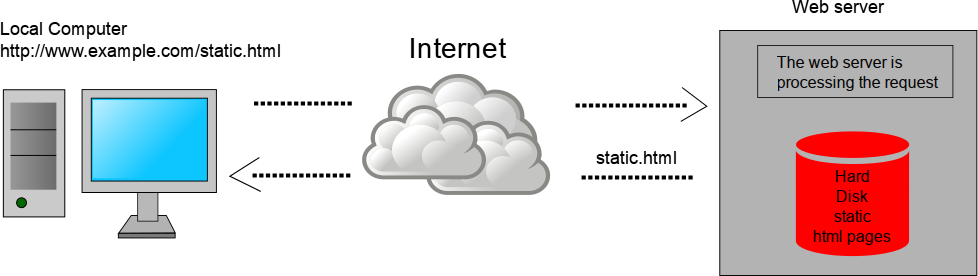
\includegraphics[scale=0.5]{Scheme_static_page_en.png}
\caption{Static web page: is delivered to the user exactly as stored.}
\label{Scheme_static_page_en}
\end{figure}


Consequently a static web page displays the same information for all users, from all contexts, subject to modern capabilities of a web server to negotiate content-type or language of the document where such versions are available and the server is configured to do so.

Static web pages are often HTML documents stored as files in the file system and made available by the web server over HTTP (nevertheless URLs ending with ".html" are not always static). However, loose interpretations of the term could include web pages stored in a database, and could even include pages formatted using a template and served through an application server, as long as the page served is unchanging and presented essentially as stored.

Static web pages are suitable for the contents that never or rarely need to be updated. However, maintaining large numbers of static pages as files can be impractical without automated tools. Any personalization or interactivity has to run client-side, which is restricting.







\chapter{Dynamic web page}




A dynamic web page\cite{dynamic_web_page} is a web page with rendered web content that varies based on parameters provided by a user or a computer program presenting content that has been customized or actualized for each individual viewing or rendition or that continually updates information as the page is displayed to the user.

\begin{figure}[!h]
\centering
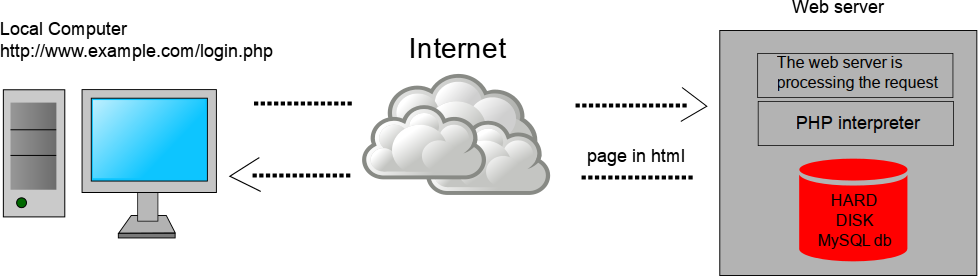
\includegraphics[scale=0.5]{Scheme_dynamic_page_en.png}
\caption{Dynamic web page: example of server-side scripting (PHP and MySQL).}
\label{Scheme_dynamic_page_en}
\end{figure}



\section{Client-side scripting}

Client-side scripting is changing interface behaviors within a specific web page in response to mouse or keyboard actions, or at specified timing events. In this case, the dynamic behavior occurs within the presentation. The Client-side content is generated on the user's local computer system.

Such web pages use presentation technology called rich interfaced pages. Client-side scripting languages like JavaScript or ActionScript, used for Dynamic HTML (DHTML) and Flash technologies respectively, are frequently used to orchestrate media types (sound, animations, changing text, etc.) of the presentation. The scripting also allows use of remote scripting, a technique by which the DHTML page requests additional information from a server, using a hidden frame, XMLHttpRequests, or a Web service

The first "widespread used" version of JavaScript was in 1996 (with Netscape 3 and ECMAScript standard).










\section{Server-side scripting}


A program running on a web server (server-side scripting) is used to generate the web content on various web pages, manage user sessions, and control workflow. Server responses may be determined by such conditions as data in a posted HTML form, parameters in the URL, the type of browser being used, the passage of time, or a database or server state.

Such web pages are often created with the help of server-side languages such as ASP, ColdFusion, JavaScript Perl, PHP, Ruby, WebDNA and other languages. These server-side languages often use the Common Gateway Interface (CGI) to produce dynamic web pages. Two notable exceptions are ASP.NET, and JSP, which reuse CGI concepts in their APIs but actually dispatch all web requests into a shared virtual machine.

Dynamic web pages are often cached when there are few or no changes expected and the page is anticipated to receive considerable amount of web traffic that would create slow load times for the server if it had to generate the pages on the fly for each request.






\section{Combination}

Ajax is a web development technique for dynamically interchanging content which sends a request to the server for data. The server returns the requested data which is then formatted by a client side script. This technique can reduce server load time because the client does not request the entire webpage to be regenerated by the server's language parser; only the content that will change is transmitted. Google Maps is an example of a web application that uses Ajax techniques.

A Web client program (such as a web browser) can access data from many different servers, such as Gopher, FTP, NNTP (Usenet) or HTTP. The HTTP server was designed specifically for the Web, and employs a protocol (system of messages) that supports sending documents from the server to a browser, and that also support sending complex data from the client back to the server. There are several HTTP methods for doing this (in HTTP, method is a technical term for the way in which data are sent between a client browser and server).

All of the client and server components that collectively build dynamic web pages for one website are together called a web application. Web applications manage user interactions, state, security, and performance.






\section{History}


It is difficult to be precise about "dynamic web page beginnings" or chronology, because the precise concept makes sense only after the "widespread development of web pages": HTTP has been in use since 1990, HTML, as standard, since 1996. The web browsers explosion started with 1993's Mosaic. It is obvious, however, that the concept of dynamically driven websites predates the internet, and in fact HTML. For example, in 1990, before general public use of the internet, a dynamically driven remotely accessed menu system was implemented by Susan Biddlecomb, at the University of Southern California BBS on a 16 line TBBS system with TDBS add-on.database.

Execusite introduced the first dynamic website solution for the professional marketplace in June 1997. Execusite was acquired by Website Pros (now Web.com) in January 2000. During the bust cycle of the Dot-com bubble, the original Execusite founders bought back the company from Website Pros (December 2000). Execusite was later acquired by Wolters-Kluwer in December 2001 and was re-branded as CCH Site Builder.





\chapter{Web Application}

In computing, a web-based application\cite{web_application} is any application that uses a web browser as a client. The term may also mean a computer software application that is coded in a browser-supported programming language (such as JavaScript, combined with a browser-rendered markup language like HTML) and reliant on a common web browser to render the application executable.


Web applications are popular due to the ubiquity of web browsers, and the convenience of using a web browser as a client, sometimes called a thin client. The ability to update and maintain web applications without distributing and installing software on potentially thousands of client computers is a key reason for their popularity, as is the inherent support for cross-platform compatibility. Common web applications include webmail, online retail sales, online auctions, wikis and many other functions.

网络应用程序(简称 Webapp)是一种使用网页浏览器在互联网或企业内部网上操作的应用软件。是一种以网页语言(例如HTML、JavaScript、Java等编程语言)撰写的应用程序,需要通过浏览器来运行。

网络应用程序风行的原因之一,是因为可以直接在各种电脑平台上运行,不需要事先安装或定期升级等程序。常见的网页应用程序有Webmail、网络商店、网络拍卖、wiki、网络论坛、博客、网络游戏等许多应用。

\begin{compactitem}
\item 网络应用程序不需要任何复杂的“展开”过程,用户所需要的只是一个适用的浏览器;
\item 网络应用程序通常耗费很少的用户硬盘空间,或者一点都不耗费;
\item 它们不需要更新,因为所有新的特性都在服务器上执行,从而自动传达到用户端;
\item 网络应用程序和服务器端的网络产品都很容易结合,如email功能和搜索功能;
\item 因为它们在网络浏览器窗口中运行,所以大多数情况下它们是通过跨平台使用的 (例如Windows,Mac,Linux等等)
\end{compactitem}



\section{History}


In earlier computing models, e.g. in client-server, the load for the application was shared between code on the server and code installed on each client locally. In other words, an application had its own client program which served as its user interface and had to be separately installed on each user's personal computer. An upgrade to the server-side code of the application would typically also require an upgrade to the client-side code installed on each user workstation, adding to the support cost and decreasing productivity.

In contrast, web applications use web documents written in a standard format such as HTML and JavaScript, which are supported by a variety of web browsers. Web applications can be considered as a specific variant of client-server software where the client software is downloaded to the client machine when visiting the relevant web page, using standard procedures such as HTTP. Client web software updates may happen each time the web page is visited. During the session, the web browser interprets and displays the pages, and acts as the universal client [3] for any web application.

In the early days of the Web each individual web page was delivered to the client as a static document, but the sequence of pages could provide an interactive experience, as user input is returned through web form elements embedded in the page markup.

In 1995 Netscape introduced a client-side scripting language called JavaScript allowing programmers to add some dynamic elements to the user interface that ran on the client side. So instead of sending data to the server in order to generate an entire web page, the embedded scripts of the downloaded page can perform various tasks such as input validation or showing/hiding parts of the page.

In 1996, Macromedia introduced Flash, a vector animation player that could be added to browsers as a plug-in to embed animations on the web pages. It allowed the use of a scripting language to program interactions on the client side with no need to communicate with the server.

In 1999, the "web application" concept was introduced in the Java language in the Servlet Specification version 2.2. [2.1?].[4][5] At that time both JavaScript and XML had already been developed, but Ajax had still not yet been coined and the XMLHttpRequest object had only been recently introduced on Internet Explorer 5 as an ActiveX object.[6]

In 2005, the term Ajax was coined, and applications like Gmail started to make their client sides more and more interactive. A web page script is able to contact the server for storing/retrieving data without downloading an entire web page.

In 2011, HTML5 was finalized, which provides graphic and multimedia capabilities without the need of client side plugins. HTML5 also enriched the semantic content of documents. The APIs and document object model (DOM) are no longer afterthoughts, but are fundamental parts of the HTML5 specification. WebGL API paved the way for advanced 3D graphics based on HTML5 canvas and JavaScript language. These have significant importance in creating truly platform and browser independent rich web applications.






\section{Interface}

Through Java, JavaScript, DHTML, Flash, Silverlight and other technologies, application-specific methods such as drawing on the screen, playing audio, and access to the keyboard and mouse are all possible. Many services have worked to combine all of these into a more familiar interface that adopts the appearance of an operating system. General purpose techniques such as drag and drop are also supported by these technologies. Web developers often use client-side scripting to add functionality, especially to create an interactive experience that does not require page reloading. Recently, technologies have been developed to coordinate client-side scripting with server-side technologies such as PHP. Ajax, a web development technique using a combination of various technologies, is an example of technology which creates a more interactive experience.








\section{Structure}

Applications are usually broken into logical chunks called "tiers", where every tier is assigned a role. Traditional applications consist only of 1 tier, which resides on the client machine, but web applications lend themselves to an n-tiered approach by nature. Though many variations are possible, the most common structure is the three-tiered application.[7] In its most common form, the three tiers are called presentation, application and storage, in this order. A web browser is the first tier (presentation), an engine using some dynamic Web content technology (such as ASP, ASP.NET, CGI, ColdFusion, JSP/Java, PHP, Perl, Python, Ruby on Rails or Struts2) is the middle tier (application logic), and a database is the third tier (storage). The web browser sends requests to the middle tier, which services them by making queries and updates against the database and generates a user interface.

For more complex applications, a 3-tier solution may fall short, and it may be beneficial to use an n-tiered approach, where the greatest benefit is breaking the business logic, which resides on the application tier, into a more fine-grained model. Another benefit may be adding an integration tier that separates the data tier from the rest of tiers by providing an easy-to-use interface to access the data. For example, the client data would be accessed by calling a "list\_clients()" function instead of making an SQL query directly against the client table on the database. This allows the underlying database to be replaced without making any change to the other tiers.


There are some who view a web application as a two-tier architecture. This can be a "smart" client that performs all the work and queries a "dumb" server, or a "dumb" client that relies on a "smart" server. The client would handle the presentation tier, the server would have the database (storage tier), and the business logic (application tier) would be on one of them or on both. While this increases the scalability of the applications and separates the display and the database, it still doesn't allow for true specialization of layers, so most applications will outgrow this model.






\section{Business use}


An emerging strategy for application software companies is to provide web access to software previously distributed as local applications. Depending on the type of application, it may require the development of an entirely different browser-based interface, or merely adapting an existing application to use different presentation technology. These programs allow the user to pay a monthly or yearly fee for use of a software application without having to install it on a local hard drive. A company which follows this strategy is known as an application service provider (ASP), and ASPs are currently receiving much attention in the software industry.

Security breaches on these kinds of applications are a major concern because it can involve both enterprise information and private customer data. Protecting these assets is an important part of any web application and there are some key operational areas that must be included in the development process.[8] This includes processes for authentication, authorization, asset handling, input, and logging and auditing. Building security into the applications from the beginning can be more effective and less disruptive in the long run.

In cloud computing model web applications are software as a service (SaaS). There are business applications provided as SaaS for enterprises for fixed or usage dependent fee. Other web applications are offered free of charge, often generating income from advertisements shown in web application interface.

Many businesses are enabled by open source web applications such as e-commerce software that facilitates easily creating an online retail store. Most businesses today do not need to buy data center hardware such as servers because they are affordably rented on a short term basis from a plethora of hosting companies that provide turnkey implementations of web applications. It is common for hosting providers to also offer packages of hardware and all necessary software to support the business needs of a company. Innovations in all aspects of web applications are providing tremendous economic value by increasing competition by reducing barriers to entry for new companies.





\section{Writing web applications}


Writing of web applications is often simplified by open source software such as Django, Ruby on Rails or Symfony called web application frameworks. These frameworks facilitate rapid application development by allowing a development team to focus on the parts of their application which are unique to their goals without having to resolve common development issues such as user management.[9] While many of these frameworks are open source, this is by no means a requirement.

The use of web application frameworks can often reduce the number of errors in a program, both by making the code simpler, and by allowing one team to concentrate on the framework while another focuses on a specified use case. In applications which are exposed to constant hacking attempts on the Internet, security-related problems can be caused by errors in the program. Frameworks can also promote the use of best practices[10] such as GET after POST.

In addition, there is potential for the development of applications on Internet operating systems, although currently there are not many viable platforms that fit this model.




\section{Applications}


Examples of browser applications are simple office software (word processors, online spreadsheets, and presentation tools), but can also include more advanced applications such as project management, computer-aided design, video editing and point-of-sale.






\section{Benefits}

\begin{compactitem}
\item Web applications do not require any complex "roll out" procedure to deploy in large organizations. A compatible web browser is all that is needed;
\item Browser applications typically require little or no disk space on the client;
\item They require no upgrade procedure since all new features are implemented on the server and automatically delivered to the users;
\item Web applications integrate easily into other server-side web procedures, such as email and searching.
\item They also provide cross-platform compatibility in most cases (i.e., Windows, Mac, Linux, etc.) because they operate within a web browser window.
\item With the advent of HTML5, programmers can create richly interactive environments natively within browsers. Included in the list of new features are native audio, video and animations, as well as improved error handling.
\item Modern web applications support greater interactivity and greatly improved usability through technologies such as AJAX that efficiently exchange data between the browser and the server.
\item Web applications allow for easier introduction of new user devices (e.g. smartphones, tablets) because they have built-in browsers.
\end{compactitem}




\section{Drawbacks}

\begin{compactitem}
\item In practice, web interfaces, compared to thick clients, typically force significant sacrifice to user experience and basic usability.
\item Web applications absolutely require compatible web browsers. If a browser vendor decides not to implement a certain feature, or abandons a particular platform or operating system version, this may affect a huge number of users;
\item Standards compliance is an issue with any non-typical office document creator, which causes problems when file sharing and collaboration becomes critical;
\item Browser applications rely on application files accessed on remote servers through the Internet. Therefore, when connection is interrupted, the application is no longer usable. However, if it uses HTML5 API's such as Offline Web application caching,[11] it can be downloaded and installed locally, for offline use. Google Gears, although no longer in active development, is a good example of a third party plugin for web browsers that provides additional functionality for creating web applications;
\item Since many web applications are not open source, there is also a loss of flexibility, making users dependent on third-party servers, not allowing customizations on the software and preventing users from running applications offline (in most cases). However, if licensed, proprietary software can be customized and run on the preferred server of the rights owner;
\item They depend entirely on the availability of the server delivering the application. If a company goes bankrupt and the server is shut down, the users have little recourse. Traditional installed software keeps functioning even after the demise of the company that produced it (though there will be no updates or customer service);
\item Likewise, the company has much greater control over the software and functionality. They can roll out new features whenever they wish, even if the users would like to wait until the bugs have been worked out before upgrading. The option of simply skipping a weak software version is often not available. The company can foist unwanted features on the users or cut costs by reducing bandwidth. Of course, companies will try to keep the good will of their customers, but the users of web applications have fewer options in such cases unless a competitor steps in and offers a better product and easy migration;
\item The company can theoretically track anything the users do. This can cause privacy problems.
\item According to Jonathan Zittrain, the online applications like Facebook and Google Apps have made the Internet become far more proprietary than early versions of Microsoft Windows.
\end{compactitem}

\begin{compactitem}
\item 网络应用程序强调浏览器的适用性。如果浏览器方没有提供特定的功能,或者弃用特定的平台或操作系统版本(导致不适用),就会影响大量用户;
\item 网络应用依靠互联网远程服务器端的应用文件。因此,当连接出问题时,应用将不能正常使用。但是,如果使用HTML5 API,这些应用就可以被下载安装而可离线使用。Google Gears,就是一个好例子;
\item 许多网络应用程序不是开源的,只能依赖第三方提供的服务,因此不能针对用户定制化、个性化,而且大多数情况下用户不能离线使用,因而损失了很多灵活性;
\item 它们完全依赖应用服务商的可及性。如果公司倒闭,服务器停止使用,用户也无法追索以前的资料。对比而看,即使软件制造商倒闭了,传统的安装软件也可以继续运行,尽管不能再更新或有其他用户服务;
\item 相似地,提供方公司对软件和其功能有了更大的控制权。只要他们愿意就能为软件添加新特性,即使用户想等bugs先被解决再更新。跳过较差的软件版本也不可能了。公司可以强加不受欢迎的特性给用户,也可以随意减少带宽来削减开支。当然,公司会尽量地讨用户欢喜——只在有竞争者提供更好的服务与方便的转接性的情况下。否则用户别无选择,只能默默承受;
\item 公司理论上可以检索任何的用户行为。这有可能引起隐私安全问题。
\end{compactitem}


\clearpage

\bibliographystyle{plainnat}
\bibliography{webdevelopment}








































\end{document}












